% !TEX root = review.tex

\subsubsection{Troullier}
\label{sssec:troullier}

Under plane-wave expansion, a wave function is
\begin{equation}
	\Psi_{\bm{k}} (\bm{r}) = \sum_{j}
	a (\bm{G}_j + \bm{k}) e^{i (\bm{G}_j + \bm{k}) \cdot \bm{r}}.
\end{equation}
Thus the Fourier transformation of semilocal potential will be
\begin{equation}
	V_l^\text{SL} (\bm{G}_j + \bm{k}, \bm{G}_i + \bm{k})
	= \frac{ 2l+1 }{ 4\pi \Omega } P_l (\cos \gamma)
	\int_{0}^{\infty} V_l^\text{SL} (r)
	J_l \Big(\abs{\bm{G}_j + \bm{k}} \bm{r} \Big)
	J_l \Big(\abs{\bm{G}_i + \bm{k}} \bm{r} \Big) r^2 \, dr,
\end{equation}
and that for K and B pure nonlocal pesudopotential will be
\begin{multline}
	V_l^\text{NL} (\bm{q}, \bm{q}')
	= \sum_{m = -l}^{l}
	\frac{ Y_{lm} (\bm{q}) Y_{lm}^\ast (\bm{q}') }{ \Omega
		\braket{ \Phi_{l} (r) | \delta V_l^\text{NL} (r) | \Phi_{l} (r) }} \\
	\int_{0}^{\infty} \Phi_{l} (r) V_l^\text{NL} (r) J_l (\abs{q r}) r^2 \, dr
	\int_{0}^{\infty} \Phi_{l} (r) V_l^\text{NL} (r) J_l (\abs{q' r}) r^2 \, dr.
\end{multline}







\citeauthor{Troullier:1991ey} improved Kerker's method \cite{Kerker:1980cs} by imposing more
terms in $p(r)$:
\begin{equation}
	p(r) = c_{12} r^{12} + c_{10} r^{10} + c_8 r^8 + c_6 r^6 + c_4 r^4 + c_2 r^2 + c_0,
\end{equation}
since they find the behavior of pesudo-wave-function can be improved by setting all odd coefficients
to be zero. Except for what Kerker did in $\eqref{eq:kerker0}$, $\eqref{eq:kerker1}$,
$\eqref{eq:kerker-pp}$ and $\eqref{eq:cond1}$,
they also derive the derivatives of $p(r)$ up to $4$th order,
combining with zero curvature of pesudopotential at origin
\begin{equation}
	\frac{ d^2 }{ d r^2 } V_l^\text{scr} (0) = c_2^2 + c_4 (2 l + 5) = 0.
\end{equation}
There are $7$ equations now, among them $5$ are linear and can be solved by Gauss--Jordan
elimination.
Then $c_i$'s can be solved and $\chi_l$ is exposed.

If the all-electron potential and an energy $\varepsilon$ is given,
then the solution of Kohn--Sham equation is uniquely defined by the
value of $\mathcal{R}(r_0)$ and it's derivate $\mathcal{R}'(r_0)$. Combine
these $2$ factors, the solution is uniquely defined by its  logarithmic
derivative
\begin{equation}\label{eq:ld}
	\frac{ d }{ dr } \ln \psi_l (r, E) \bigg|_{r = r_0}
	= \frac{ 1 }{ \psi_l (r, E) }
	\frac{ d }{ dr } \psi_l (r, E) \bigg|_{r = r_0},
\end{equation}
where $\psi = R(r)$, the pseduo-radial-wave-function, or
$\psi = \mathcal{R}$, the all-electron wave-function.

Since Friedel sum rule,\cite{Topp:1973cp}
\begin{equation}\label{eq:friedelsr}
	- 2\pi \bigg[ \big(r \psi_E(r) \big) ^ 2 \frac{ d }{ dE } \frac{ d }{ dr } \ln \psi_E(r) \bigg]_{ r = R_c} = 4\pi \int_{0}^{R_c} r^2 \abs{\psi_E(r)}^2 \, dr = Q,
\end{equation}
and the charge $Q$ of pesudo-wave-function and $\mathcal{Q}$ of
wave-function are equal when talking about norm-conserving pesudopotential,
thus within to a region surrounding $\epsilon_l$,
equation
\begin{equation}\label{eq:tmcri}
	\frac{ 1 }{ R_l (r, \epsilon) }
	\frac{ d }{ dr } R_l (r, \epsilon)
	=
	\frac{ 1 }{ \mathcal{R}_l (r, \varepsilon) }
	\frac{ d }{ dr } \mathcal{R}_l (r, \varepsilon)
\end{equation}
is closely satisfied,
\cite{Troullier:1991ey} think this means all-electron
wave-function and pesudo-wave-function are proportional outside $R_c(l)$.
Thus, they think $\eqref{eq:tmcri}$ is a good criterion for quickly testing
the quality of the pesudopotential, i.e., they compare the
logarithmic derivative $\eqref{eq:ld}$ of all-electron wave-function and pesudo-wave-function as a function of $\varepsilon$ outside $R_c$.

\begin{figure}[H]
	\centering
	\begin{minipage}[t]{.46\linewidth}
		\centering
		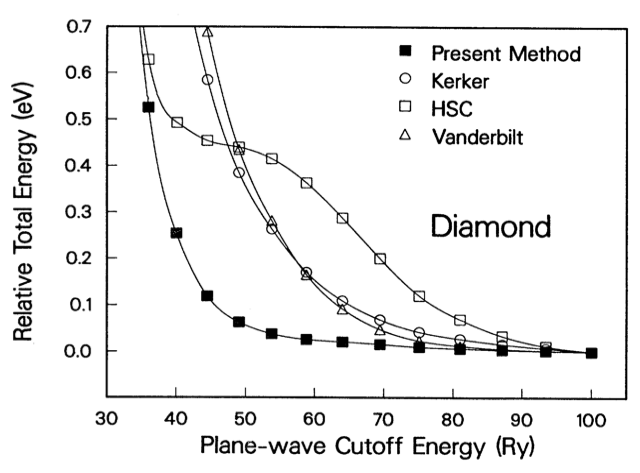
\includegraphics[width=\linewidth]{tmfig1}
		\caption{Total energy for diamond per primitive cell vs cutoff energy
			of the plane-wave basis set. All four curves are referenced at a total
			energy calculated at a cutoff energy of \SI{100}{Ry}.
			\cite{Troullier:1991ey}}
		\label{fig:tm-e:a}
	\end{minipage}%
	\hfil
	\begin{minipage}[t]{.46\linewidth}
		\centering
		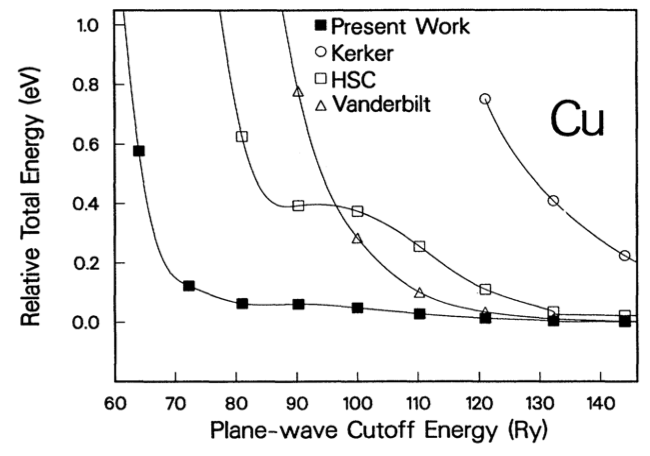
\includegraphics[width=\linewidth]{tmfig8}
		\caption{Total energy for FCC \ce{Cu} vs the cutoff energy
			of the plane-wave basis set. All four curves are referenced at a total
			energy calculated at a cutoff energy of \SI{225}{Ry}.
			\cite{Troullier:1991ey}}
		\label{fig:tm-e:b}
	\end{minipage}
\end{figure}
A smoother pesudopotential implies a faster convergence in
total energy, and therefore a more rapid convergence in system properties.
\citeauthor{Troullier:1991ey} compared $4$ pesudopotential methods'
results. A large enough cutoff energy is chosen and set as a reference.
From Fig. \ref{fig:tm-e:a} and Fig. \ref{fig:tm-e:b} we can see that their
total energy converges faster than that of HSC, Kerker and Vanderbilt's.
From Fig. \ref{fig:tm-8:a} and Fig. \ref{fig:tm-8:b} we can also see that
faster energy convergence do not need a more rapid pesudopotential
convergence in Fourier space, and \emph{vice versa}.
An depth of pseudopotential is also not a good convergence indicator,
since the slower convergence can be from shallower pesudopotential (HSC for \ce{C})
or from deeper pesudopotential (Kerker for \ce{Cu}).
For \ce{Cu}, they use KB procedure and set $s$ potential as local component.
The exchange-correlations are both \citeauthor{ceperley1980ground}'s method which parametrized by \citeauthor{perdew1981self}.
\begin{figure}[H]
	\centering
	\begin{minipage}[b]{.7\linewidth}
		\centering
		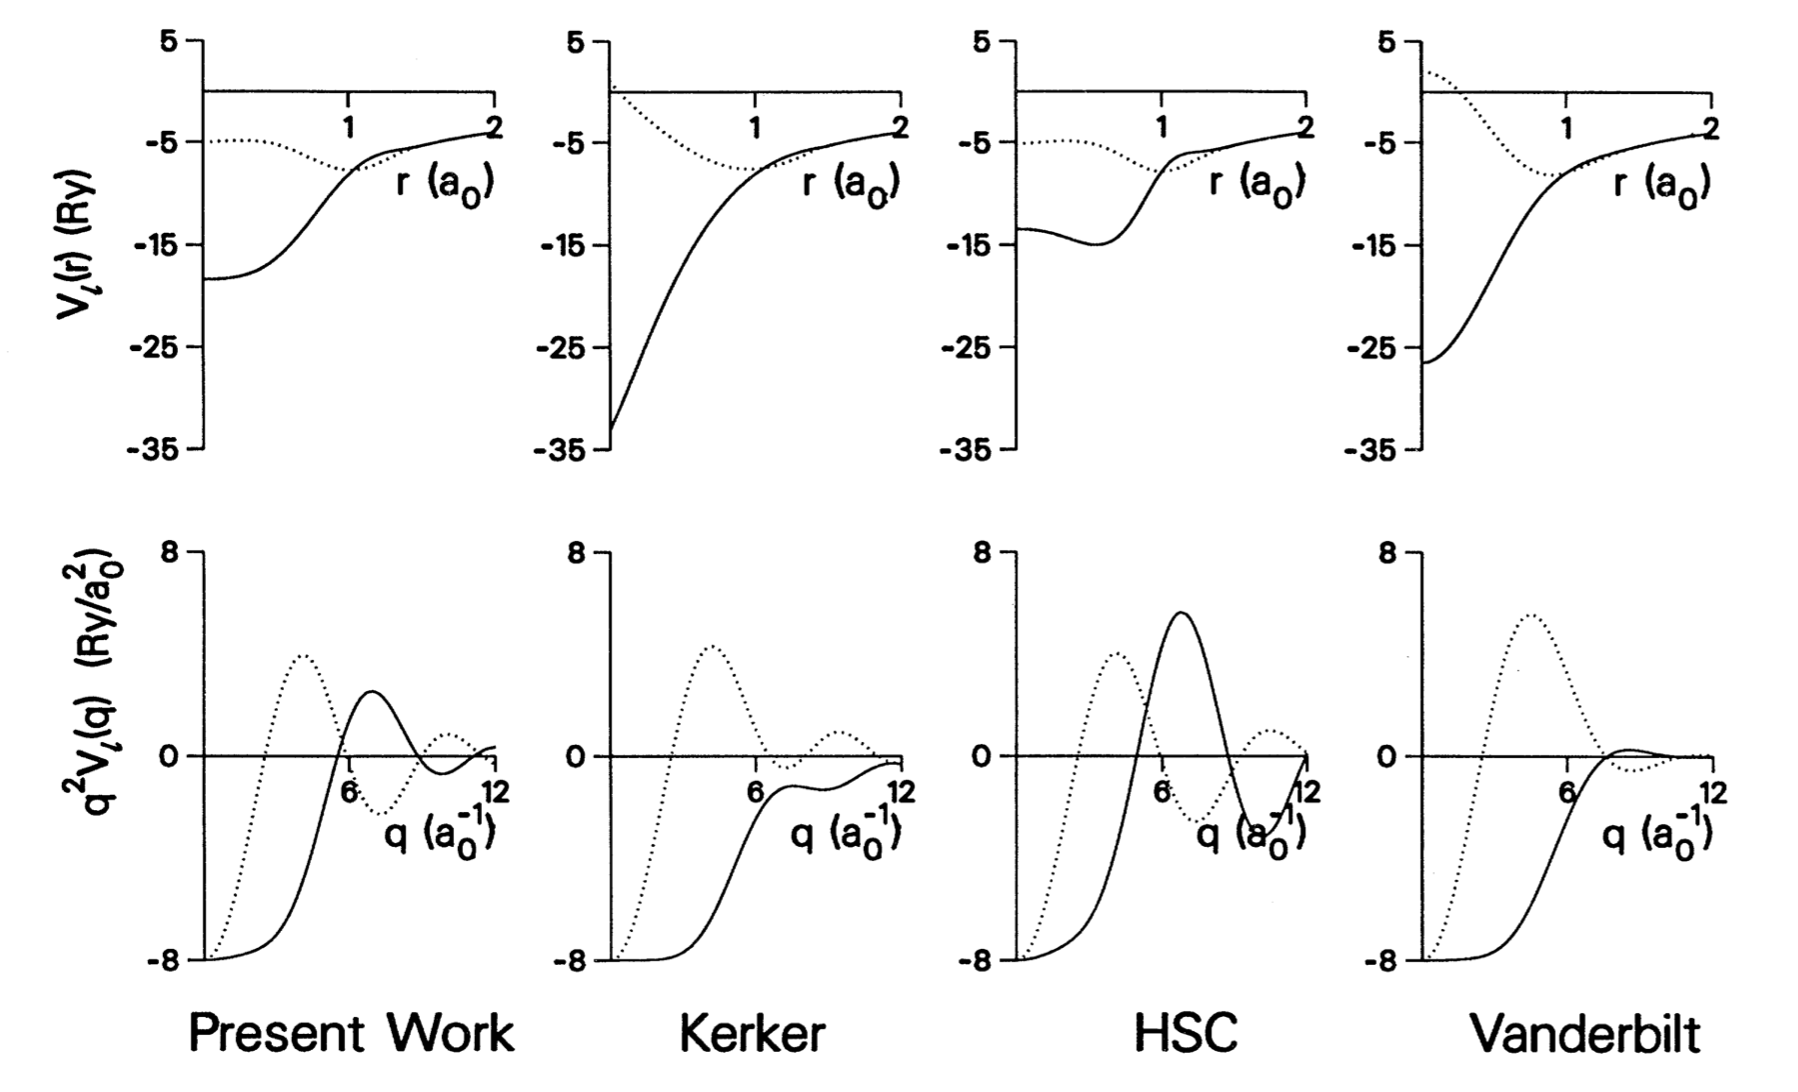
\includegraphics[width=\linewidth]{tmcarbon}
		\caption{Ionic pesudopotential for \ce{C} using $4$ schemes in both real and Fourier space.
			The dotted and solid curves correspond to the $s$ and $p$ pseudopotentials, respectively.
			\cite{Troullier:1991ey}}
		\label{fig:tm-8:a}
	\end{minipage}%
	\vspace{\baselineskip}
	\begin{minipage}[b]{.7\linewidth}
		\centering
		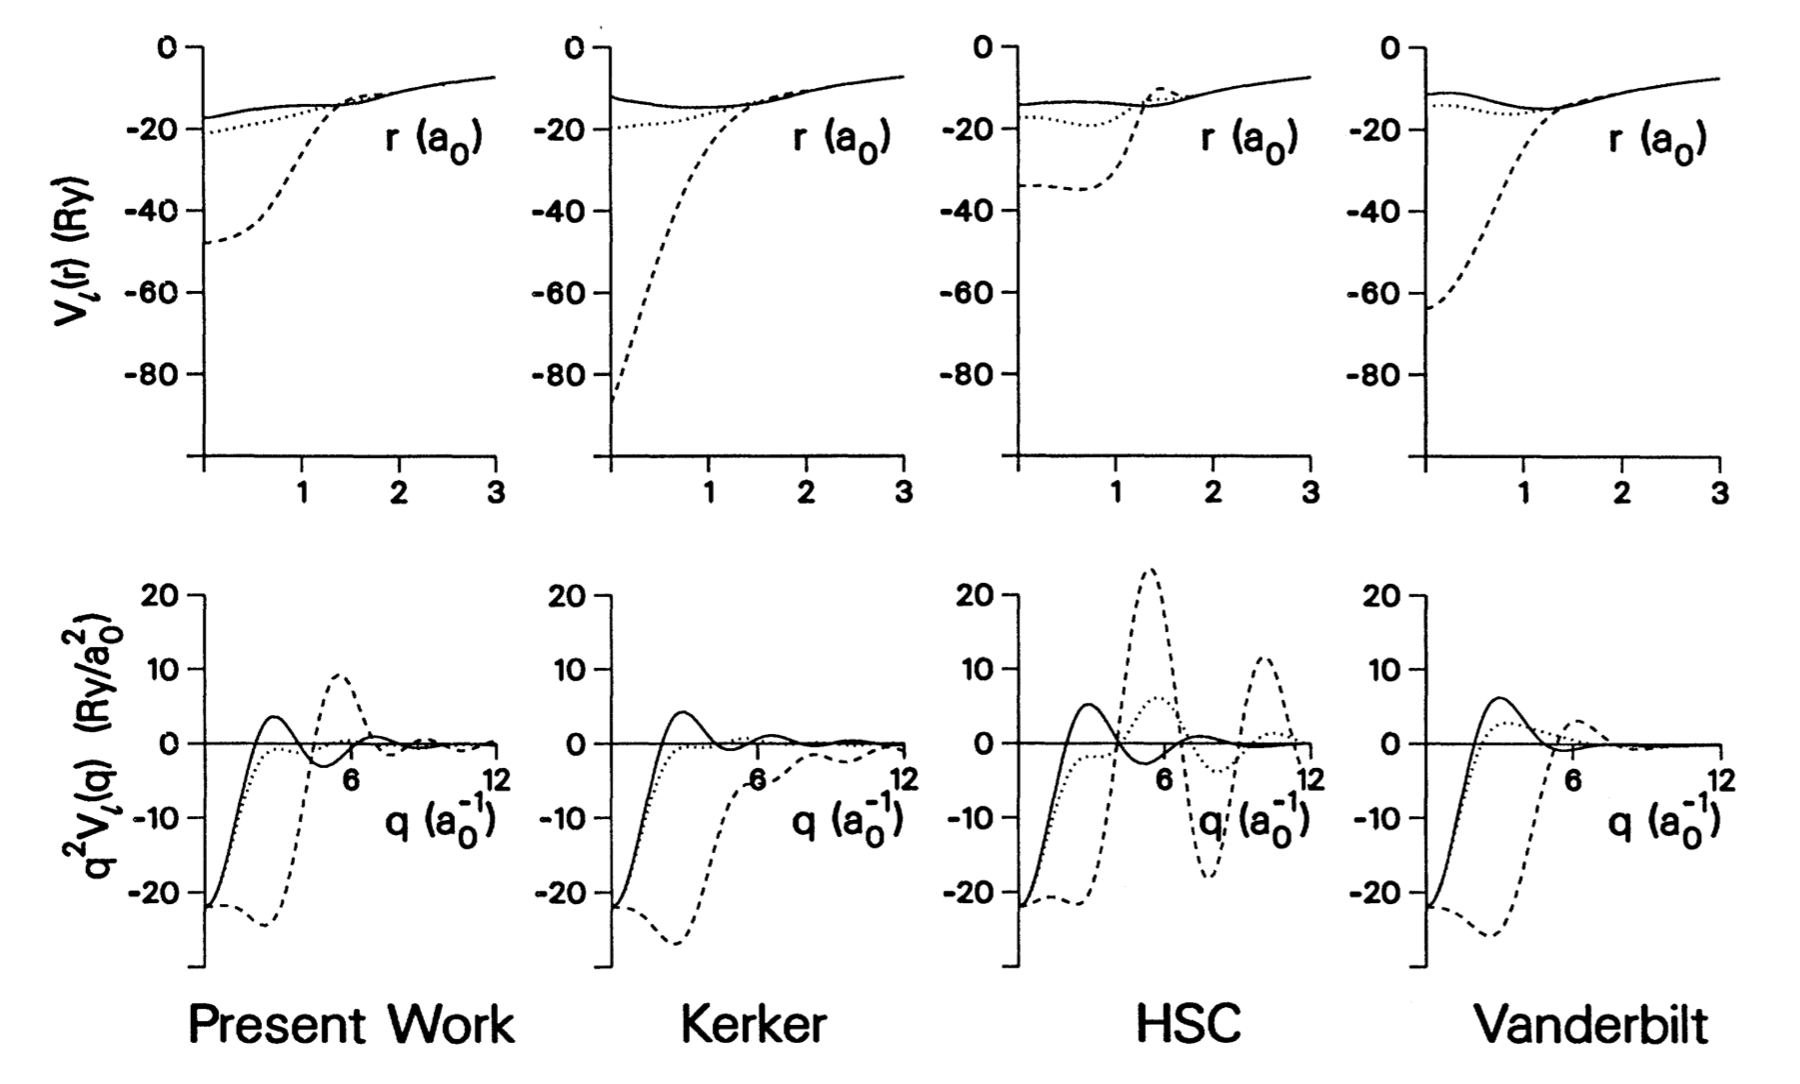
\includegraphics[width=\linewidth]{tmcu}
		\caption{Ionic pesudopotential for \ce{Cu} using $4$ schemes in both real and Fourier space.
			The dotted and solid curves correspond to the $s$ and $p$ pseudopotentials, respectively.
			\cite{Troullier:1991ey}}
		\label{fig:tm-8:b}
	\end{minipage}
\end{figure}

The authors also plotted a figure,
see Fig. \ref{fig:tmfig6} for reference,
comparing logarithmic derivatives of pesudo-wave-function and all-electron
wave-function for \ce{Cu}. We need to supplement that the cutoff radii $R_c(l)$
chosen in Fig. \ref{fig:tm-8:a} and Fig. \ref{fig:tm-8:b} are all done using this way,
i.e., the logarithmic energy derivatives of pesudo-wave-functions math that of all-electron wave-functions.
\begin{figure}[H]
	\centering
	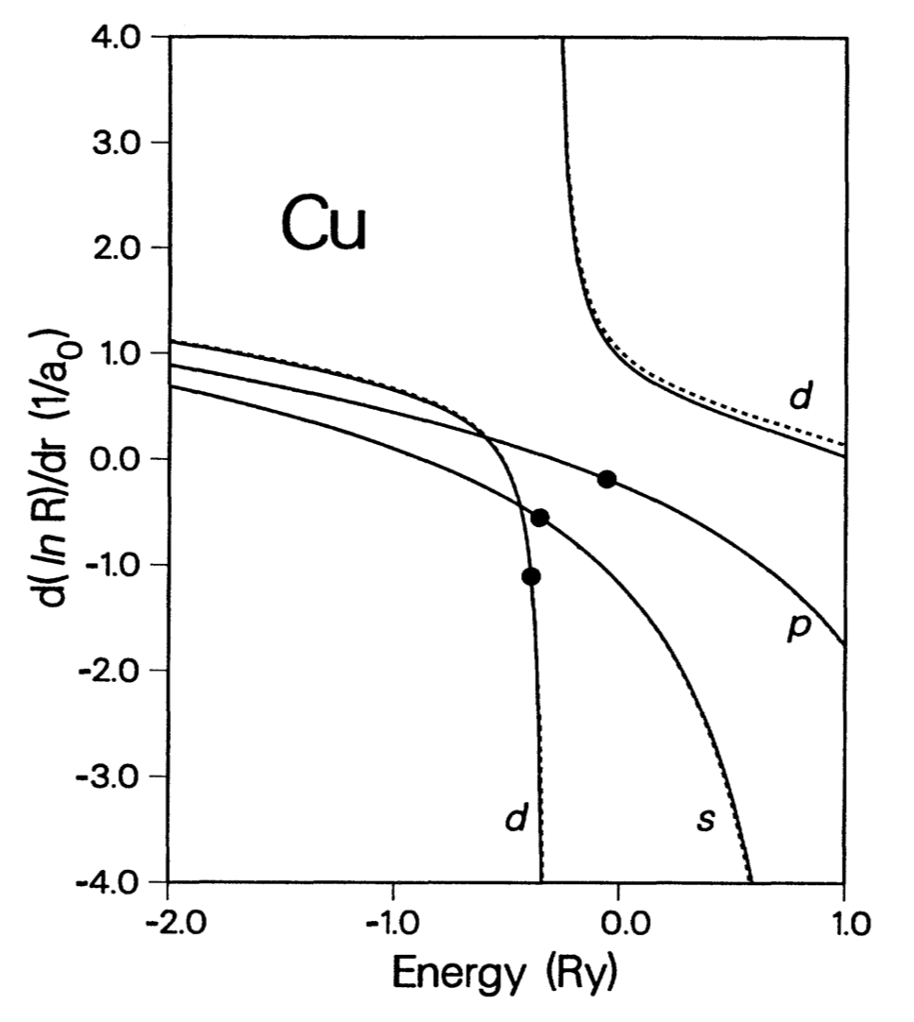
\includegraphics[width=0.4\linewidth]{tmfig6.png}
	\caption{The comparison of logarithmic derivatives of pesudo-wave-function
		and all-electron wave-function at $r = \SI{2.6}{\bohr}$, they coincide very well. The black points are eigenvalues.
		The slop is logarithmic energy derivatives shown in $\eqref{eq:friedelsr}$.
		It shows good transferability and no ghost state of KB pesudopotential.}
	\label{fig:tmfig6}
\end{figure}